%RELATED

\subsection{Multiple Instance Learning}

The Multiple Instance Learning (MIL) problem was first described by Dietterich in the context of drug activity prediction \cite{dietterich97}. In this problem, we want to figure out which of a number of different molecules will bind to a target ``binding site". Each molecule can assume a number of different 3-dimensional shapes, so even for molecules that are known to bind to the binding site, it is not necessarily known which formation of the molecule succeeds in binding. If even one shape of a given molecule binds to the binding site, it is considered a ``good" molecule \cite{dietterich97}. Thus, in the original formation of MIL, a bag is classified as positive if one or more instances within it is positive, while a negative bag contains only negative instances. This is commonly referred to as the ``standard multiple instance assumption" \cite{amores13}. In the original paper, Dietterich develops a solution based on axis-parallel rectangles to solve this problem, and the MIL approach was shown to be significantly more effective than a standard supervised learning approach \cite{dietterich97}. In the late 1990s and early 2000s, a number of different approaches were developed for the original MIL problem, such as Diverse Density (DD) \cite{perez98}, EM-DD \cite{zhang01}, MI-SVM \cite{andrews02}, sbMIL \cite{bunescu07}, and MILES \cite{wang06}. A recent review of MIL by Amores created a taxonomy of these various methods and compared their effectiveness for classification \cite{amores13}. Most of these classic methods follow the standard assumption, which is not useful in real domains in which negative bags may contain some positive instances.
%

More recently, there has been increased interest in different formulations of the MIL problem. For instance, the problem of ``key instance detection" \cite{zhou12} revolves around finding the instances that contribute the most to bag labels. A recent study focused on a formulation of the MIL problem in which bags with negative labels can contain some positive instances, and developed a general cost function for determining individual instance labels from group labels \cite{kotzias15}. This is significant in metagenomics because, while some diseases are caused by a single pathogen, many arise from a combination of many factors, and even patients that are healthy may contain small amounts of pathogens that are normally associated with disease. In contrast with the standard assumption, this can be referred to as the ``collective" assumption \cite{amores13}. Additionally, it is helpful to discover which microbes and which functional attributes of those microbes lead to disease, making instance level information significant in this domain.
%

While some of the above methods follow the standard assumption and others follow the collective assumption, they all treat bag labels simply as aggregations of instance labels and thus focus only on comparisons between individual instances and not entire bags or groups of instances. For methods following the standard assumption, the aggregation function is simply an OR function: if any of the instances in a bag are positive, the entire bag is positive. For methods following the collective assumption, the aggregation function is often based on an averaging of instance labels. Regardless of the problem assumption, methods that rely only on comparisons between individual instances are referred to as ``Instance Space" by Amores, and he showed that this paradigm was generally significantly less effective than the two other paradigms, ``Bag Space" and ``Embedded Space" \cite{amores13}. Bag Space methods define a distance or kernel function that determine the similarity between bags, while Embedded Space methods map bags into feature vectors which can then be used for classifiers \cite{amores13}. Embedded Space methods can be further divided into two subcategories: methods that simply aggregate information about all instances in a bag without differentiating them, and ``Vocabulary-based" methods that group certain similar instances together and then use those groups to form the feature vector \cite{amores13}. We use a vocabulary-based method in this paper, because having information about groups of similar sequence reads can be biologically important, as explained further in the clustering section.

An example of Vocabulary-based methods are Bag of Words (BoW) methods, which involve the following three-step process: (i) Cluster the instances to create classes of instances; (ii) for each bag, map the clusters of instances in that bag to a feature vector; and (iii) use a standard classifier that uses the feature vectors to predict group labels \cite{amores13}. Amores found the Distance-based Bag of Words (D-BoW) method to be the second most effective of all tested methods, and the most effective one that was also time-efficient (linear, rather than quadratic, in the number of bags and number of instances per bag) \cite{amores13}. The distinguishing feature in D-BoW methods is that the values for the feature vector represent the instance that has the smallest distance to the cluster center. Histogram-based Bag of Words (H-BoW) methods count the number of instances from each cluster there are in each bag, instead of keeping track of the closest-matching instance to that cluster. This intuitively has appeal in the domain of microbiome analysis, as the relative quantities of different species of bacteria is important. H-BoW methods were found by Amores to be somewhat less effective than D-BoW methods on average, but performed the best out of all algorithms on several datasets, indicating that this method performs very well on real problems that it is well-suited for \cite{amores13}. The D-BoW and H-BoW feature extraction methods are illustrated as part of Figure \ref{pipeline}.

As we have discussed, the Multiple Instance paradigm fits phenotype prediction well, since we have a set of labeled patients containing unlabeled sequence reads, and we would like to predict both the patient phenotype and which reads are indicative of that phenotype. Despite the recent developments in MIL and its potential utility in phenotype prediction, we have not found any literature that specifically applies MIL to classifying patient phenotype based on metagenomic data.

\subsection{Assembly}

\begin{figure}[h]
\centering
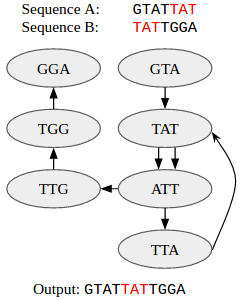
\includegraphics[scale=0.5]{./de-bruijn.png}
\caption{This diagram illustrates a basic de Bruijn graph, as explained in the text. Notice the double arrow from TAT to ATT, allowing a path to go through that route twice. Thus, the longest contig that can be created by following a path is GTATTATTGGA, which is what we want.} \label{de-bruijn}
\end{figure}

The \emph{assembly} problem involves combining overlapping short reads (usually less than 1000 base pairs) into longer sequences called \emph{contigs} (often tens of thousands of base pairs). For instance, if one read ends with the same relatively large nucleotide string that another read starts with, the reads are likely to be overlapping fragments from the same genome, and can thus be combined into one contig. This can be done either \emph{de novo} (in an unsupervised manner) or by referencing sequences against known contigs. We focus on de novo assembly, because we wish to keep our pipeline as unsupervised as possible. 

One of the main purposes of assembly is to determine the whole genomes of microbial species, the vast majority of which have not or cannot be laboratory cultured, from sequencing reads \cite{zerbino08}. Even if full genomes cannot be assembled, combining reads into larger contigs can still make them much more useful for clustering and classifiers, because the contigs will contain more phylogenetic and functional information than short reads. This is because short reads of less than 1000 base pairs constitute only a tiny fraction of microbial genomes, which are usually hundreds of thousands to millions of base pairs, making it difficult to ascertain much about the phylogeny of individual reads. Many modern sequence reads are produced by Next-Generation and High-Throughput Sequencers, which usually produce these short reads. Metagenomics additionally poses its own set of challenges, due to very large datasets and lack of knowledge about how many species are present and in what relative abundances \cite{namiki12}. Thus, metagenome assembly is a relatively new and challenging field.

Some of the popular genome and metagenome assembly approaches include SOAPdenovo2 \cite{luo12}, IDBA-UD \cite{peng12}, Velvet \cite{zerbino08}, MetaVelvet \cite{namiki12}, ABySS \cite{simpson09}, and Ray Meta \cite{boisvert12}. We used SOAPdenovo2 in our study, because it was the assembler used in the original MGWAS study \cite{qin041012} and because it has been shown to be one of the fastest assembly algorithms \cite{peng12}. SOAPdenovo2 first constructs a type of directed graph called a \emph{de Bruijn} graph that represents the overlaps between different sequences \cite{li10}. Reads are divided into strings of length K called \emph{k-mers}; these k-mers are the nodes of the graph \cite{zerbino08}. The choice of K is up to the user, and is important for having good assembly results. The k-mer nodes in the graph have an edge between them if a read contains those k-mers in order with an overlap of K-1 nucleotides, and the direction of the edge indicates in which order the k-mers appear \cite{zerbino08}. SOAPdenovo2 then cleans this graph by removing nodes/sequences with few or no connections with other sequences, eliminating ``tips" that represent likely sequencing machine errors, and removing redundant edges \cite{li10}. This step helps to reduce the overall size of the data by eliminating some reads that would not have been useful anyway. The contigs are then formed by combining reads according to the de Bruijn graph: each contig represents a directed path in the graph \cite{zerbino08}. There are variations on how exactly de Bruijn graphs are represented and implemented, but Figure \ref{de-bruijn} illustrates the general process.

\subsection{Clustering}

\begin{figure}[h]
\centering
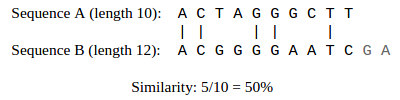
\includegraphics[scale=0.5]{./uclust-similarity.png}
\caption{This diagram illustrates the similarity computation between two sequences in UCLUST. Terminal characters are excluded, so the length of the reads is 10. In the first 10 characters of each string, there are 5 matching characters that are in the same position in the string. Thus, the similarity is 5/10 = 50\%.} \label{uclust-similarity}
\end{figure}

The \emph{clustering} problem in this context  involves grouping input short reads  such that reads within a group are similar to each other. The clusters obtained from this process are referred to as Operational Taxonomic Units (OTUs). OTUs represent a group of equivalent or similar organisms. Accordingly, the number of OTUs in a sample gives an approximation of the species diversity in that sample  \cite{schloss2009introducing,schloss2005introducing,sun2009esprit}.
In addition to approximating species diversity, clustering has several other key advantages. Because clustering is always de novo (unsupervised), it is not limited by the species that are covered in taxonomic databases. This detail is important, because it is believed that most microorganisms that reside in the human body have not been laboratory cultured \cite{handelsman04}. Clustering also reduces computational costs by allowing analyses to operate on entire clusters instead of on each read. Finally, clustering helps the classification process by allowing feature vectors to be built at the OTU level, instead of using individual short reads that contain little biological information.

UCLUST \cite{Edgar10}, CD-HIT \cite{Li01072006}, mothur \cite{schloss2009introducing}, DOTUR \cite{schloss2005introducing}, CROP \cite{Hao01032011}, MC-MinH \cite{sdm2013a}, and 
MC-LSH \cite{bibm2012} are some of the popular sequence clustering approaches. We use UCLUST within our study, which is one of the most widely used and cited metagenome clustering methods and has been shown to be amongst the most effective in terms of speed and accuracy in benchmarking studies \cite{bonder090112, sun042711}. 
%

UCLUST seeks to ensure that, for some similarity T, the following conditions hold: (i) all cluster centroids have a similarity of less than T to each other; and (ii) all points in a cluster have a similarity of greater than T to the cluster centroid \cite{Edgar10}. Thus, each \emph{centroid} defines the center of a cluster, and the distance T defines the radius of the cluster, such that any point that has a similarity of greater than T to the centroid is within the radius and is thus part of the cluster. UCLUST is a heuristic algorithm that has several optimizations to improve speed, thus condition (i) above is not always guaranteed \cite{Edgar10}. UCLUST proceeds in a greedy, iterative manner. The first sequence in the input file becomes a new cluster centroid. For each new sequence in the file, it is compared with each of the existing cluster centroids in order. As soon as it is compared with a centroid that it has a similarity of greater than T with, it becomes part of that cluster. If the read is not similar enough with any of the existing cluster centroids, it becomes the centroid of a new cluster. The similarity measure T is defined as a string similarity between the two nucleotide sequences that counts the number of character placements that they have in common and then divides that number by the length of the reads, with terminal characters excluded \cite{Edgar10}. This is illustrated in figure \ref{uclust-similarity}.